\chapter{fMRI Data Analysis} \label{ch-1}

\section{Problem Definition}

Functional Magnetic Resonance Imaging (fMRI) is the most widely applied method to image human cognition. In it, neural hemodynamics are imaged in three dimensional space, over a fourth dimension of time. In task fMRI, participants additionally engage in an in-scanner experiment designed to engage some aspect of cognition. Of interest to neuroscientists are the observed topological and, increasingly, dynamical patterns associated with the given cognitive state. While fMRI has illuminated the `neural signatures' underlying many aspects of cognition, others, such as social cognition, remain elusive.

In recent years, neuroscientists have attempted to better capture true variability in human cognition. Larger and more representative imaging studies are increasingly the norm, boasting hundreds or even thousands of participants, often conducted across multiple research centers. These investigations have reported large individual differences in anatomical \cite{kanai2011structural} and functional networks, the latter in both the spatial \cite{mueller2013individual} and temporal domains \cite{davison2016individual}. Moreover, consensus evidence shows that task fMRI captures not only task-related cognition, but also background activity, physiological processes, and motion, as well as a variety of artifacts associated with scanner hardware \cite{liu2016noise}. In short: the observed fMRI signal represents a noisy amalgam of signals of varying and often unknown provenance.

Several Factor Analysis (FA) methods have been proposed to compensate for functional variability among subjects. For instance, Shared Response Model (SRM) \cite{srm} provides a means of aligning participants’ activation via a shared low dimensional response and subject-specific bases, and Hierarchical Topographic Factor Analysis (HTFA) \cite{htfa} learns a global template of brain activity and casts each participant’s response as a perturbation of that template. However, these methods are limited in that they treat time as static, though converging evidence suggests that temporal correlation structure -- even on the slow timescale of hemodynamics -- carries meaningful signal \cite{infraslow}. Gaussian Process Factor Analysis (GPFA) \cite{gpfa} accommodates time by linking together factor analyzers in low-dimensional latent space, using imposed Gaussian process priors. This allows GPFA to model temporal and spatial structure in observation space, and has been applied within subjects to model dynamic functional connectivity \cite{lfgp}: an initial proof of principle of its suitability to fMRI.

\section{Background}

Shared Response Model (SRM) \cite{srm} is a multi-view extension of probabilistic Principal Component Analysis (pPCA) \cite{ppca}, wherein latent factors (named the shared response) are common across all subjects for each time point, while fixed factor loadings are specific to each subject. In addition, SRM explicitly imposes an orthogonality constraint on its loading matrices. Variants of this model such as Robust Shared Response Model (RSRM) \cite{rsrm} have been proposed in which both shared and private components in subjects' responses are explicitly modeled, similar to probabilistic Canonical Correlation Analysis (pCCA) \cite{pcca}. Similarly, in \cite{lukic2002ica} an ICA-based method has been proposed to separate shared and private sources in subjects' fMRI observations based on a similar factor model by exploiting time delayed correlations.

Similar to static dimensionality reduction methods like Linear Factor Analysis (LFA) and PCA, SRM treats multivariate time series of fMRI recordings as a collection of independent snapshots in time, entirely disregarding temporal information. In other words, SRM remains invariant if training time series are shuffled through the time dimension. As with PCA, SRM cannot discover temporal dynamics unless such dynamics materialize as variance, which stems from both dynamics and noise \cite{dca}. 

Moreover, to address the rotational ambiguity of latent variables and factor loadings, SRM adopts a similar solution as PCA, by enforcing subjects' factor loadings to be orthonormal. Although this restricts the output to be unique, the resulting solution may not be interpretable since the assumption of orthogonal topographies is likely an undue simplification of physiology. Nonetheless, SRM's solution captures the shared structures in subjects' fMRI observations. An alternative solution for resolving rotational ambiguity is to utilize the inherent temporal dynamic of the data. This can address the aforementioned problems at once, i.e. finding unique and interpretable solutions whilst bringing insight about shared dynamic structures in observations. We adopt a similar approach as in Gaussian Process Factor Analysis (GPFA) \cite{gpfa}, where latent variables are linked through time by employing Gaussian Process priors, allowing viable modeling of both temporal and spatial covariance in data.

Closely related to S-GPFA, the family of Matrix Normal SRM \cite{mnsrm} models temporal dynamics of fMRI data by imposing a Matrix-Normal prior over shared timeseries. However, S-GPFA does not impose a Kronecker-separable covariance structure over shared timeseries, and hence, is not in the family of matrix-variate normal models. Instead, S-GPFA models independent latent temporal components that can unfold over different timescales, effectively discovering components of diverse temporal scales. In MN-SRM however, the same temporal covariance structure is assumed over different components of the shared space.

\section{The Proposed Model: Shared-GPFA}
\label{sec:sgpfa}

In the following, we present the mathematical formulation of the probabilistic model for S-GPFA. We denote by $\A_{i,:}$, $\A_{:, j}$, and $[\A]_{m,n}$ the $i$th row vector, the $j$th column vector, and element $(m, n)$ of matrix $\A$, respectively. Let $\Y{m} \in \reals^{\q \times \t}$ be the observed high-dimensional fMRI time series for subject $m \in \{1, 2, \ldots, \m \}$ where $\q$ is the number of voxels (or in general, brain regions), $\t$ is the number of time samples (in TRs), and $\m$ is the total number of subjects in the dataset. We denote by $\Y{m}_{q,:} \in \reals^{1\times \t}$ the $q$-th row of the observation matrix, or equivalently, the time series of brain activation in region $q$ for subject $m$. We assume all subjects are exposed to identical and time-synchronized stimuli while brain activities are recorded and activation time series are centered over time.
S-GPFA extracts shared low-dimensional latent trajectories $\X \in \reals^{\p \times \t}$ describing the common latent state of all subjects, where their linear combinations through loading matrices of each subject describe the observed activation time series.
Here, $\p$ is a hyperparameter to be set as the dimensionality of the latent space ($\p < \q$). 
Following the standard Factor Analysis model, we define a set of linear (isotropic) Gaussian systems for fMRI observations and latent trajectories:

\begin{equation}
    \Y{m}_{:, t} | \X_{:, t}\, , \w{m} \sim \mathcal{N} \left( \w{m} \X_{:, t}, \spcov{m} \right)
\end{equation}

where $\w{m} \in \reals^{\q \times \p}$ and $\spcov{m} \in \reals^{\q \times \q}$ denote the factor loading matrix and observation noise covariance matrix for subject $m$, respectively. Note that columns of factor loadings can be considered as brain activation bases meant to capture subject-specific topographies (we use the terms `factor loadings' and `subject topographies' interchangeably). Constraining $\spcov{m}$ to be diagonal will let $\w{m}$ and $\X$ completely define the covariance structure of region activation patterns.
% The $q$th diagonal element in $\spcov{m}$ represents the independent noise variance of region $q$ in subject $m$.
To explicitly let brain region $q$ of subject $m$ accommodate different noise levels, we model the diagonal elements as $[\spcov{m}]_{q, q} = \sv{m} \rv{q}$, where $\rho$ and $\sigma$ are subject-specific and region-specific learnable parameters, respectively. Following standard GPFA, to model the temporal correlation of the data, we impose independent Gaussian Process (GP) priors over latent trajectories:

\begin{equation}
    \X_{p, :} \sim \mathcal{GP}\left(0, \kappa_p(\cdot , \cdot) \right), \hspace{1.5em} p \in \{1, \ldots, \p\}
\end{equation}

where $\kappa_p$ denotes a Mercer kernel function. Therefore, the covariance matrix for the $p$th latent trajectory, $\K_p$, will be the Gram matrix of the kernel over the index set $\{1, 2, \ldots, \t\}$, i.e. $[\K_p]_{t_1,t_2} = \kappa_p(t_1, t_2)$. In general, the choice of kernel function imposes important assumptions on the form and smoothness of observed time series. Following prior literature \cite{infraslow,lfgp}, we opt to employ commonly-used Squared Exponential (SE) kernel functions:

\begin{equation}
    \kappa_p (t_1, t_2) = \alpha_p^2 \exp \left( -\frac{(t_1 - t_2)^2}{2\tau_p^2} \right) + \eta_p^2 \, \mathds{1}_{t_1=t_2}
\end{equation}

Hence, the GP prior is fully parameterized through the kernel variance $\alpha_p^2$, characteristic timescale $\tau_p \in \reals_+$, and the kernel independent noise variance $\eta_p^2$. Furthermore, we fix the scale of $\X$ to have $\X_{:,t} \sim \mathcal{N}(0, I)$ by setting $\alpha_p^2 + \eta_p^2 = 1$. This will prevent the identifiability issue in the scale of $\X$ and $\w{m}$ by allowing unconstrained learning for factor loadings \cite{gpfa,infraslow,lfgp}. We also set $\eta_p^2$ to a small value to act as a diagonal jitter for numerical stability. Therefore, the characteristic timescales $\tau_p$ can fully define the priors over latent trajectories. Figure \ref{fig:model} shows the graphical model for S-GPFA along with the summary of model specification.

% S-GPFA models within and between-subjects temporal and spatial covariance in a fMRI dataset: 
% \begin{equation}
%     \operatorname{Cov} \left( \Y{m_1}_{q_1, t_1} , \Y{m_2}_{q_2, t_2} \right) = \sum_{p=1}^{\p} \w{m_1}_{q_1,p} \w{m_2}_{q_2,p} \kappa_p(t_1, t_2) + \delta_{m_1, m_2} \delta_{q_1, q_2} \delta_{t_1, t_2} \rv{q_1} \sv{m_1}
%     % \operatorname{Cov} \left( \Y{m}_{q, t} , \Y{m'}_{q', t'} \right) = \w{m}_{q,:} [] \w{m'}_{q',:}^T + \delta_{m, m'} \delta_{q, q'} \delta_{t, t'} \rv{q} \sv{m}
% \end{equation}

\begin{figure}[t]
    \begin{minipage}{.5\textwidth}
        \centering
        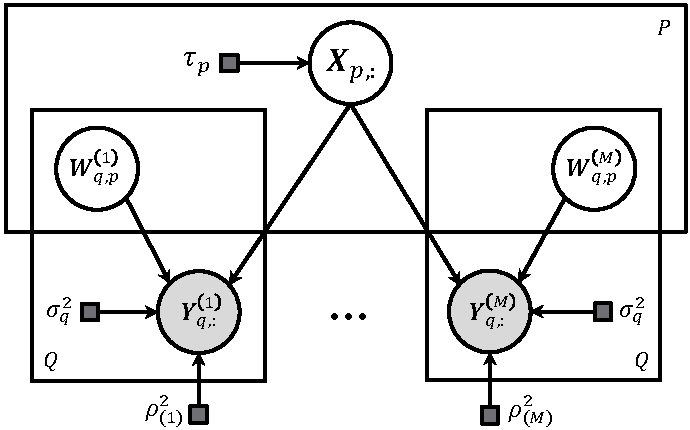
\includegraphics[width=.8\linewidth]{figures/ch1/unfold_M.pdf}
        \caption{\footnotesize Graphical Model for S-GPFA.} \label{fig:model}
    \end{minipage}
    \begin{minipage}[c]{.5\textwidth}
        \savebox\strutbox{$\vphantom{\dfrac11}$}
        \begin{align*}
            & \X_{p, :} \sim \mathcal{GP}\left(0, \kappa_p(.,.) \right) \\
            & \w{m}_{q,p} \sim \mathcal{N}(0, 1) \\
            & \Y{m}_{:, t} | \X_{:, t}, \w{m} \sim \mathcal{N} \left( \w{m} \X_{:, t}, \spcov{m} \right) \\
            & \kappa_p(t_1, t_2) = \exp \left( -\frac{(t_1 - t_2)^2}{2\tau_p^2} \right)
        \end{align*}
  \end{minipage}
    \vspace{-1em}
\end{figure}

\sloppy To find the model parameters, we employ gradient ascent (using ADAM optimizer \cite{adam} and TensorFlow Probability) to maximize the joint probability distribution of observations and latent variables, conditioned on model parameters. The collective set of model parameters and latent variables to be inferred is denoted by $\params=\Bigl\{ \X, \{\w{m}, \sv{m}\}_{m=1}^M, \{\rv{q}\}_{q=1}^Q, \{\tau_p\}_{p=1}^P \Bigr\}$. The resulting maximum a posteriori (MAP) estimate of model parameters is the minimizer of the objective function in (\ref{eq:nll}):

\begin{align} \label{eq:nll}
    % \hat\params = & \underset{\params}{\operatorname{argmin}} \nonumber \\
    & \sum_{m=1}^{M} \sum_{q=1}^{Q} \left[ \frac{T}{2} \log(2\pi\sv{m}\rv{q}) + \frac{\norm{ \Y{m}_{q,:} - \w{m}_{q,:} \X }^2}{2\sv{m}\rv{q}} \right]   \\
    + & \frac{\lambda}{2} \sum_{p=1}^{P} \left[\log\det(2\pi \K_{p}) + \X_{p,:} \K_{p}^{-1} \X_{p,:}^T \right]
    % \nonumber \\
    + \sum_{m=1}^{M} \frac{1}{2} \norm{\w{m}}_F^2 
     \nonumber
\end{align}

where $\norm{\cdot}_F$ denotes the Frobenius norm. For now, let us set $\lambda=1$ to achieve the standard MAP solution -- we will explain the motivation behind including such constant in the objective function later in this section. The first summation term in (\ref{eq:nll}) is the reconstruction loss promoting data fit. We refer to the second summation term as the smoothness loss, where $\log\det(\K_p)$ constitutes a model complexity penalty (in terms of smoothness) and $\X_{p,:} \K_{p}^{-1} \X_{p,:}^T$ promotes smooth latent trajectories governed by $\tau_p$. Finally, the last term is a weight decay loss for subjects' factor loadings. While the reconstruction loss favors complex models to fit the observed data, smoothness and loadings weight decay losses act as regularizers to promote smooth and less flexible models, respectively.

Increasingly, fMRI studies include sample sizes of hundreds of participants ($M$) with thousands of voxels recorded ($Q$). An examination of the objective function in (\ref{eq:nll}) reveals that the objective is extensively dominated by the reconstruction loss, since the total number of observed time series, $Q M$, is often orders of magnitudes larger than the latent space dimensionality $P$. In such a case, the solution of (\ref{eq:nll}) cannot afford to model the temporal smoothness properties of the data, and consequently, attempts to fit the observed data with a possibly complex model. To resolve this issue, we amplify the smoothness loss in (\ref{eq:nll}) by hyperparameter $\lambda \propto \m\q/\p$ to balance the weight of the smoothness loss against the reconstruction loss. Note that from a probabilistic perspective, such regularization can be interpreted as weighted likelihood \cite{weightedlikelihood}. Although, as with any hyperparameter, standard methods like cross validation can be employed to tune $\lambda$, we use the fixed value of $0.1 \times \m\q/\p$ for all experiments conducted in the present paper. 

\sloppy Adding a new subject $\m+1$ to a previously trained model is done through finding the maximizer of $\text{P}(\Y{\m+1}, \w{\m+1} | \X, \sv{\m+1},  \{\rv{q}\}_{q=1}^Q)$ with respect to $\w{\m+1}$ and $\sv{\m+1}$. Note that the shared latent trajectories, existing subject's topographies, and region/subject noise factors will remain unchanged.
In addition, using previously learned topographies, shared timescales, and noise factors, one can map new observations from the existing subjects in the training cohort into the shared space. This can be done by maximizing 
$\text{P}(\{\y_{\text{new}}^{(m)}\}_{m}, \X_{\text{new}} | \{\w{m}, \sv{m}\}_{m}, \{\rv{q}\}_{q=1}^Q, \{\tau_p\}_{p=1}^P)$
with respect to $\X_{\text{new}}$, where $\y_{\text{new}}$ denotes new observations from the subjects in the training cohort and $\X_{\text{new}}$ shows the associated shared latent trajectories. 


\section{Results}
\label{sec:experiments}

We present two sets of experiments to demonstrate the utility of S-GPFA. First, using the Raider datasets \cite{ha}, we perform the time segment matching experiment to measures generalization of learned temporal dynamics and topographies to unseen subjects and observations. In the second experiment, we apply our model to another multi-subject dataset (SPINS \cite{spins}), allowing us to evaluate and interpret topographies and group-specific temporal dynamics. 
% Further details of both datasets has been published by original study authors \cite{ha, spins}.
% Taken together, our experiments show the proposed model can achieve equal performance in terms of aggregating subjects' observations, by employing temporal information already available in data, without the need for imposing unrealistic modeling assumptions. 

\subsection{Time Segment Matching}
A time segment matching experiment, as first introduced by \cite{ha}, can evaluate how shared dynamics found by S-GPFA generalizes to new subjects and unseen data. We follow the modified version of the experiment presented in \cite{srm}, where the task is to locate an unseen segment of a test subject's response in time. We partition the fMRI dataset in time into two equal-size parts and leave one subject out to use the remaining subjects as training participants. We shall note the four resulting parts as \ytrain{1}, \ytest{1}, \ytrain{2}, and \ytest{2}.

As shown on the top diagram in Figure \ref{fig:tsm}, the first half of the data is used to learn subject-specific topographies. First, an S-GPFA model is fit to the first half of training subjects' data \ytrain{1}, to learn shared latent trajectories \xtrain{1} and subject-specific topographies \wtrain. Next, using the learned shared trajectories \xtrain{1} and the first half of test subject's data \ytest{1}, topographies for the held-out subjects \wtest is calculated, as discussed in section \ref{subsec:model}. The second half of data is used for measuring time segment matching accuracy. More specifically, given the second half of training subjects' data, \ytrain{2}, we wish to locate an unknown segment from the held-out subject's data \yseg in time. By only using the raw observations as a baseline, one can first find the average response of training subjects, then report the time where \yseg and the average response are maximally correlated. Moreover, using learned subject topographies, we can transform \ytrain{2} and \yseg into the shared space using \wtrain and \wtest as discussed in section \ref{subsec:model}, to find \xtrain{2} and \xseg. Using a similar correlation classifier, we can locate the test segment in the point where \xtrain{2} and \xseg are maximally correlated. Figure \ref{fig:tsm} compares the time segment matching accuracy for different query segment lengths. S-GPFA demonstrates similar performance as SRM in terms of time segment matching accuracy. This posits that shared temporal dynamics (timescales) found in training subjects can be generalized to new subjects with unseen observations. 

\begin{figure}[tb!]
    \centering
    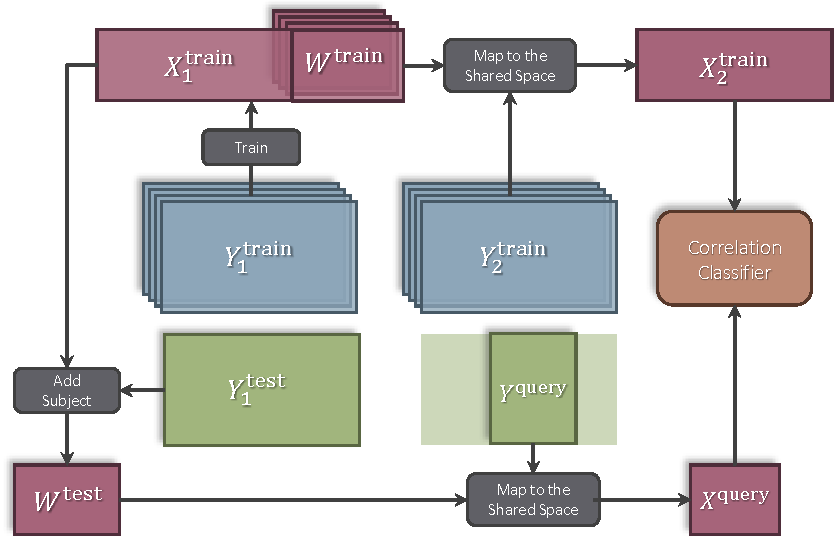
\includegraphics[width=.5\linewidth]{figures/ch1/tsm_blockdiagram.pdf}
    \vspace{1em}
    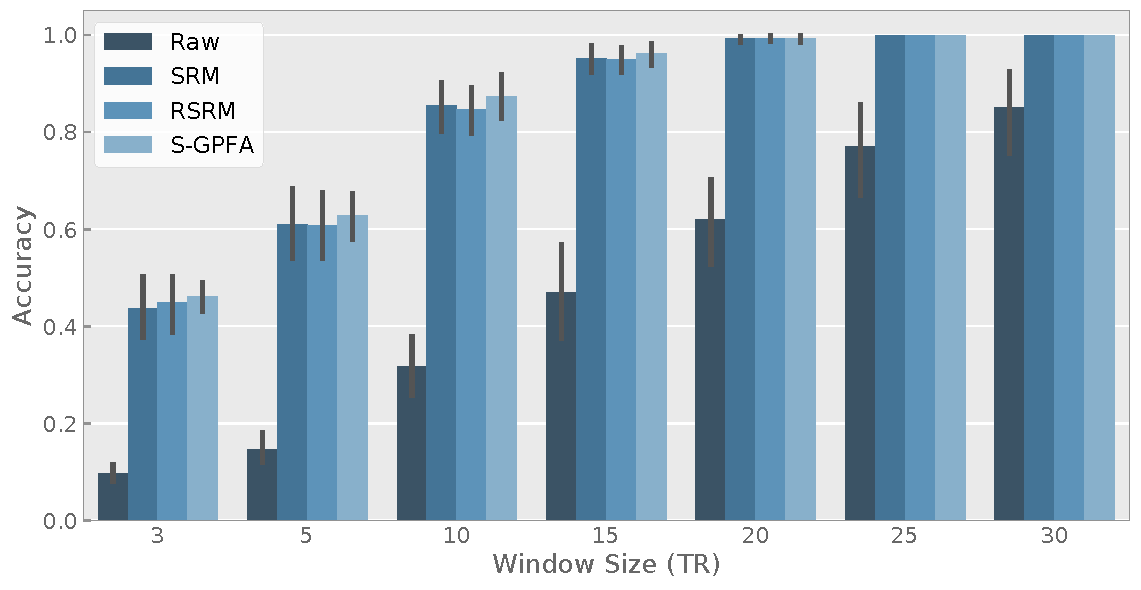
\includegraphics[width=.6\linewidth]{figures/ch1/tsm_raider_p10_sm200_2.pdf}
    \caption{Time Segment Matching Experiment. Top: schematic procedure of the experiment. Bottom: Time segment matching accuracy for Raider dataset (10 subjects, first 400 TRs). We used $P= 10$ for SRM, RSRM, and S-GPFA. Error bars show $\pm$ standard deviations.}
    \label{fig:tsm}
\end{figure}

\subsection{Application: SPINS Dataset}

\begin{figure*}[!t]
    \centering
    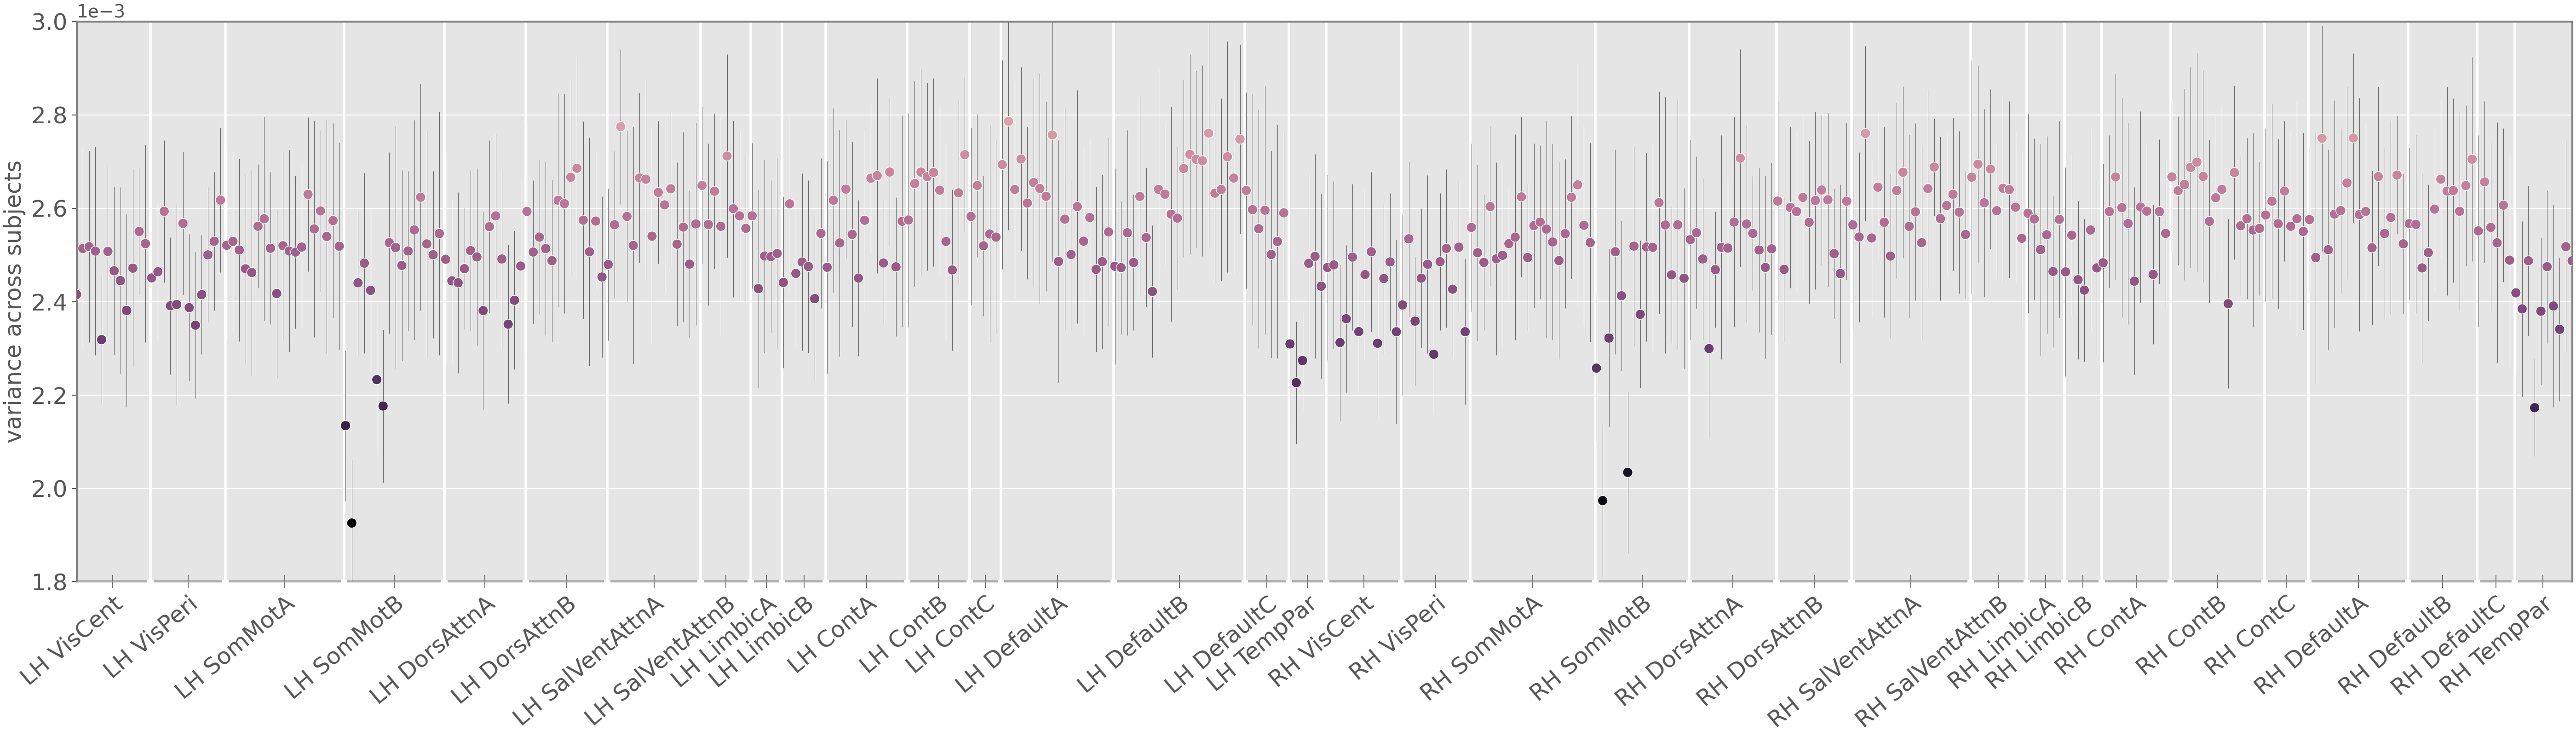
\includegraphics[width=1\linewidth]{figures/ch1/topo_cons_scatter.png}
    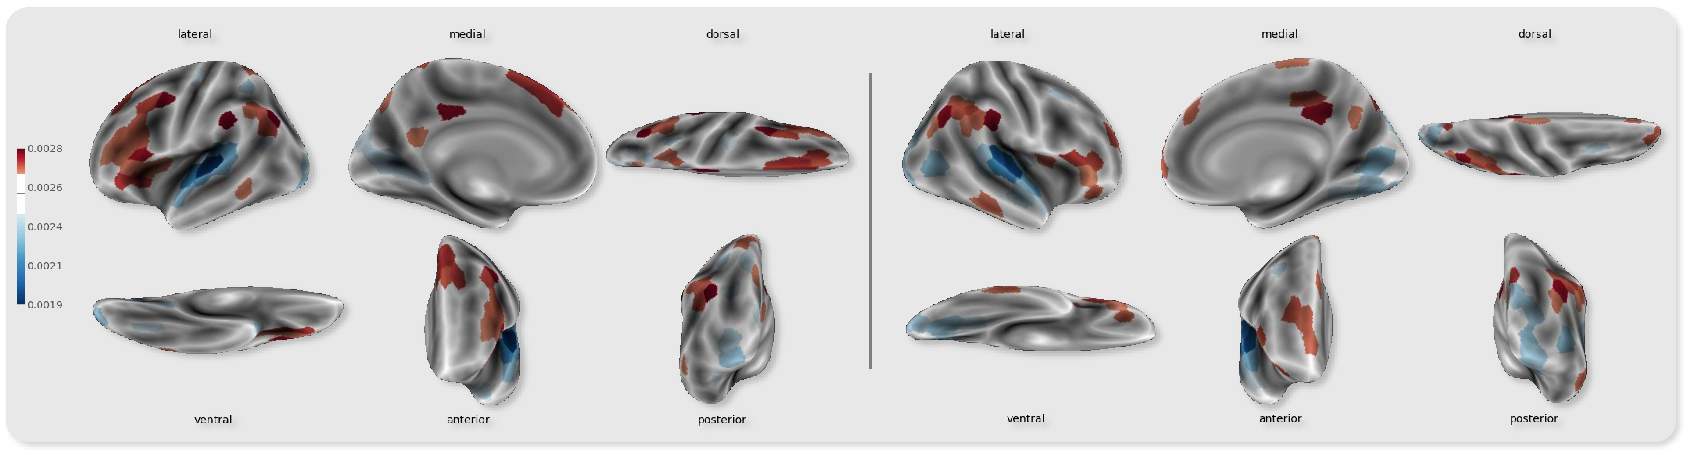
\includegraphics[width=1\linewidth]{figures/ch1/topo1_brain.pdf}
    \caption{Top: Variance of normalized $\p=20$ topographies across subjects (Y axis) for different regions (X axis). Regions are divided into 17 Yeo sub-networks \cite{yeo}. Colored dots indicate the mean (across different topographies) of variances for each region, and error bars shows $\pm$ standard deviation. Bottom: Brain surface plots of average variance of normalized topographies, for left and right hemispheres. Blue (red) indicates higher (lower) consistency across subjects. 
    % In both panels, the second of nine EA videos is shown: all videos showed comparable patterns.
    % See Supplementary Materials (section \ref{sec_suppmat:topo_consistency}) for other EA videos.
    }
    \label{fig:topo}
\end{figure*}

For our final set of experiments, we applied S-GPFA to a subset (332 subjects) from the NIMH Data Archive study “Social Processes Initiative in the Neurobiology of the Schizophrenia(s)” (SPINS) who completed the Emotional Accuracy (EA) task. The EA task collects fMRI as participants watch videos of an actor (‘target’) recounting autobiographical events. In total, 9 videos were shown, lasting for between 2-2.5 minutes. Participants provide ratings of the target’s valence on a 9-point scale (1=extremely negative, 9=extremely positive) in real time via button press. The tasks' primary dependent measure, the EA score, is the correlation between the participant’s ratings of the targets’ emotions, and the “gold standard” rating of the targets’ ratings of their own emotions, calculated in 2 second time epochs. We selected SPINS as an experimental dataset because it includes participants with and without schizophrenia, and we held that the anticipated variability in brain structure, function, and cognitive performance would provide an interesting test of S-GPFA.

\textbf{Consistency of Functional Topographies - }
In our first analysis, we examined whole-brain variation in activation during the EA task, across all subjects. Learned factor loading matrices $\W$ in S-GPFA are, by model definition, subject-specific basis vectors that generate each subject's observation from a shared set of latent trajectories: $\w{m}\X \simeq \Y{m}$. Therefore, columns of factor loadings $\{\W_{:,p} \in \reals^\q\}_{p=1}^{\p}$, for different subjects, are perturbed versions of an activation template. This allows the model to capture functional variability across subjects. Hence, we can examine the amount of subject variability in each individual brain region of interest (ROI) for a given task, by looking at the variance of learned topographies over participants. To this end, for every topography $p$ of subject $m$, we first normalize $\w{m}_{:,p}$, then we find the variance of these normalized topographies over subjects. This will result in $\p$ variance values for each of $\q$ regions indicating a measure of subject variability, as shown in Figure  \ref{fig:topo}. Note that, for the present analysis, we used cortical parcellations from the Schaefer atlas (400 ROIs) \cite{schaefer2018local} grouped in accordance with the Yeo17 parcellation \cite{yeo}. 

Examination of subject variance in functional topography itself shows variability across ROIs. Perhaps unsurprisingly, the lowest variance (blue) is evident in the motor network, engaged similarly by the task’s continuous button-press demands, and in temporal lobe areas related to audition, engaged by the audio aspect of the task. Excitingly, we see lower consistency (red) in the distributed frontal-parietal (‘Control A’) network, which contains the inferior frontal gyrus (IFG) and inferior parietal lobule (IPL), that together constitute the canonical human mirror neuron system \cite{iacoboni2006mirror}. That we were able to identify high variability in a network believed to subserve social cognition provides an important proof of principle that S-GPFA is able to identify meaningful variance within a heterogeneous sample. We expect that S-GPFA will enable important tests of both exploratory and hypothesis-driven examinations of functional topography in psychiatric disorders.

\begin{figure}[tb]
    \centering
    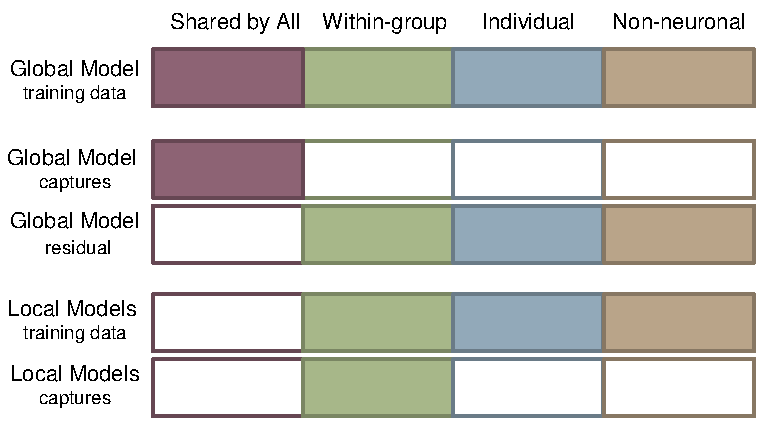
\includegraphics[width=.5\linewidth]{figures/ch1/group_tf_schematic_2.pdf}
    \vspace{0.4em}
    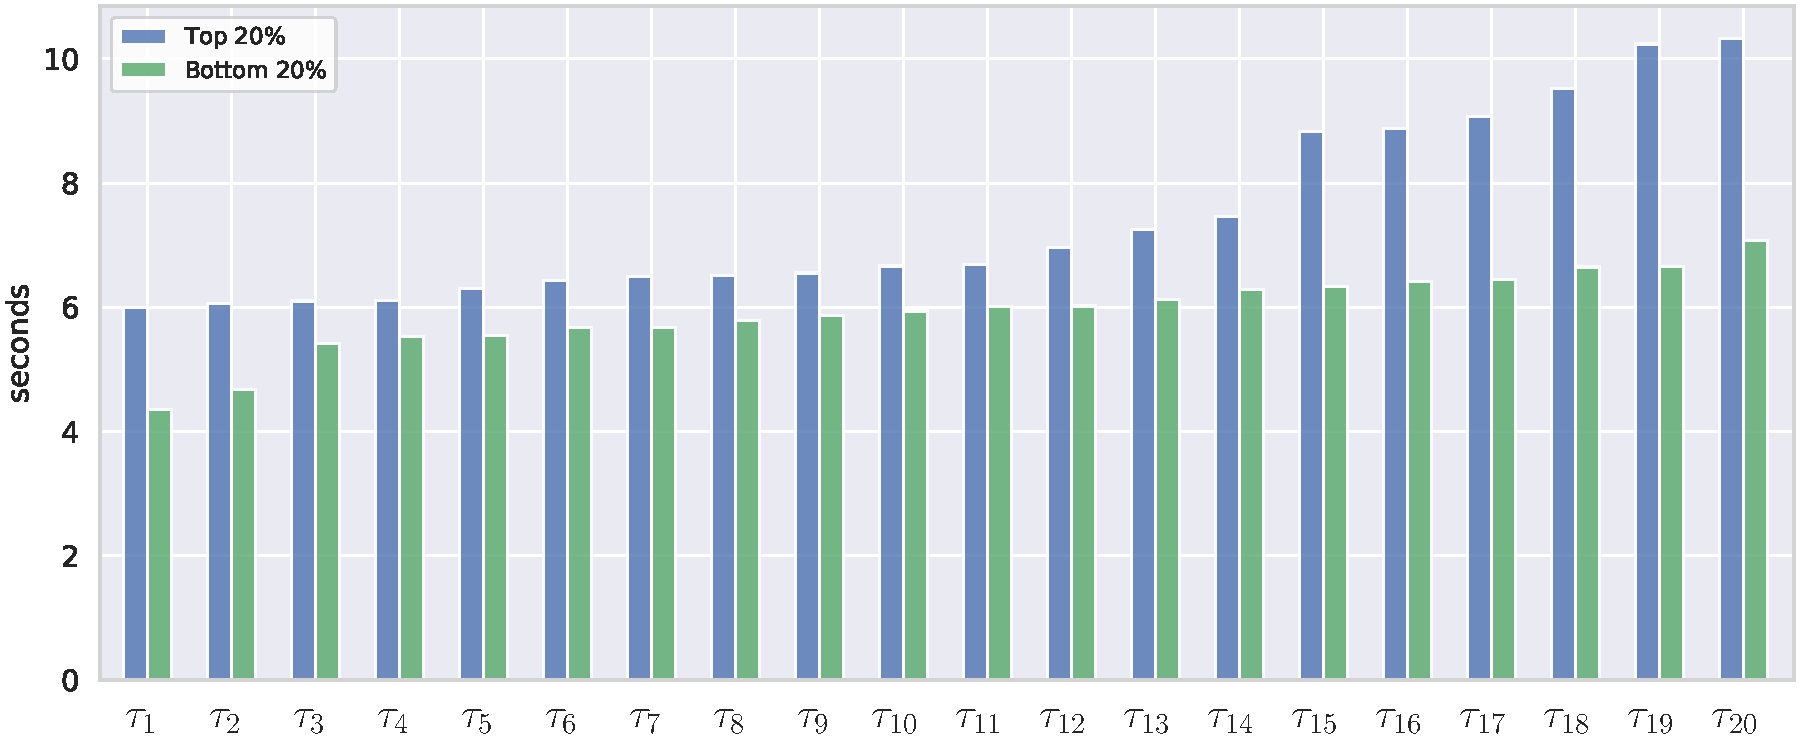
\includegraphics[width=0.9\linewidth]{figures/ch1/group_td.pdf}
    \caption{Top: Different data components captured using the global and local models. Bottom: Group-specific timescales (sorted by magnitude) discovered using local models, after removing temporal patterns shared across all subjects.}\label{fig:gtd}
\end{figure}

\textbf{Group-specific Temporal Dynamics - }
Next, we employed S-GPFA to examine group-specific temporal dynamics. Our method is illustrated in Figure \ref{fig:gtd} (top). First, a \textit{global} model is trained using subjects from all groups. Residuals of the global model, as defined by $\Y{m} - \w{m} \X$, for $m \in \{1, \ldots, \m \}$, allow us to remove components of the observations that are shared among all groups \cite{srm}. Next, separately on each group, two models are trained over the residuals of the global model. These \textit{local} models capture group-specific dynamical components in observations after the globally shared components of the data are removed. 

We applied this approach to the SPINS dataset, opting to split the sample into two smaller groups comprised of individuals demonstrating EA scores within the top and bottom 20th percentiles, respectively. This bifurcation allowed us to isolate subjects with distinctly strong and poor socioemotional cognition, irrespective of schizophrenia diagnosis \cite{insel2014nimh}. Figure \ref{fig:gtd} (bottom) shows group-specific timescales discovered via the local models, after extraction of the residuals from the global model, i.e., after all signals with a global structure have been removed. In the local models, we observe that the group with the strongest EA performance shows less temporal variability, i.e., the dynamical patterns in those individuals with the greatest socioemotional cognitive capacity unfolded over slower timescales, in contrast to those participants with comparatively impoverished capacity. This observation is consistent with broad evidence of a relationship between domain-specific task performance, and observed modularity versus flexibility of task-relevant brain networks, e.g.\cite{olsen2013functional}, and the recent dissociation that strong performance on tasks involving little executive function or cognitive control (consistent with EA task demands) may be subserved by modular network activation \cite{ramos2017static}. Importantly, the isolation of low-dimensional group-specific timescales allows for the identification of differences of small effect, which may be statistically occluded in global models. 




\section{Future Plans}